\section{Лабораторна робота 1. ООП засобами Java. Серіалізація}
 

Аудиторний час на виконання лабораторної роботи --- 16 годин.

Мета роботи полягає у набутті практичних знань та навичок. 
До знань належать:
\begin{enumerate}
\item розуміння змінних, примітивних (цілих, дійсних, булевих), непримітивних (об’єктів, масивів, перелічуваних) типів даних та операторів над ними;
\item правила допустимого іменування змінних;
\item область видимості змінних;
\item зарезервовані імена (ключові слова); 
\item принципи переозначення методів в класах-нащадках;
\item принципи поліморфізму;
\item поняття серіалізації-десеріалізації (маршалінгу-демаршалінгу).
\end{enumerate}

До практичних навичок належать:
\begin{enumerate}
\item Створення виконуваних класів, їхньої компіляції та виконання в середовищі JDK.
\item Створення класів, що інкапсулюють поля різних типів.
\item Реалізація принципу агрегації за допомогою масивів.
\item Реалізація принципу поліморфізму за допомогою похідних класів (ключові слова {\bf extends, super, this}, анотація {\bf @Override}).
\item Реалізація бінарної серіалізації стандартними засобами J2SE: інтерфейс {\bf Serializable}, методи {\bf writeObject, readObject} класів {\bf OutputStream, InputStream}. 
\end{enumerate}

\subsection{Постановка задачі}
Слід розробити консольний (J2SE) додаток, в якому обов’язково повинно бути не менше двох класів, оголошених в різних файлах. Один з цих класів повинен бути виконуваним, а інший --- класом-моделлю (структурою даних).

Виконуваний клас повинен створити масив об’єктів модельного класу, встановлюючи їхні поля у випадкові значення, а потім висвітлити їх на екрані.

\subsection{Теоретичні відомості}
Основою будь-якої прикладної програми у Java є виконуваний клас. Виконуваним вважається клас, який є загальнодоступним (public), тобто видимим за межами власного пакету (докладніше про пакети і видимість --- згодом), а також містить статичну функцію
\begin{lstlisting}
public static void main(String[]a){/* code */}
\end{lstlisting}
або
\begin{lstlisting}
public static void main(String a[]){/* code */}
\end{lstlisting}
або
\begin{lstlisting}
public static void main(String ...a){/* code */}
\end{lstlisting}

У лістингу 1 наведено приклад простого виконуваного класу.

{\bf Лістинг 1.
Приклад виконуваного класу }
\begin{lstlisting}
public class Welcome{
    public static void main(String...a){
        System.out.println("Welcome, dear "+
            "third-form students of PZAS!");
    }
}
\end{lstlisting}
Первинний код класу можна підготувати у будь-якому текстовому редакторі, навіть у notepad, хоча суттєво зручніше працювати у редакторі, що виділяє мовні конструкції кольором, наприклад, Notepad++ або у інтегрованому середовищі розробки, наприклад, Eclipse чи IntelliJ IDEA. Проте, майте на увазі, що це повинен бути справді текстовий редактор (англійською plain text editor), а не текстові процесори на зразок MS Word, які добавляють до текстів спеціальні символи форматування.
Імена файла та виконуваного класу, що в ньому знаходиться повинні співпадати. Файл мусить мати розширення ``.java''. Наприклад, первинний код виконуваного класу з лістингу 1 повинен бути збереженим будь-де у файлі з назвою Welcome.java. 
Компіляція первинного коду у байт-код, придатний до виконання віртуальною машиною Java (JVM) можна здійснити у середовищі розробки або з командного рядка.

Якщо Ви вирішили працювати у середовищі Ecilpse чи IDEA, то запустіть його. Ми рекомендуємо користуватися IntelliJ IDEA Community Edition для розробки під JavaSE та Android Studio для розробки під Android, оскільки вони мають хороші засоби інспекції коду, рефакторингу, використовують сучасну технологію збирання gradle з репозиторіями модулів повторного використання maven. 

Створіть новий проект, клацнувши на кнопку Create New Project.
Вкажіть ``App by <Ваше прізвище>'' як назву проекту. Звісно вставте Ваше справжнє прізвище замість <Ваше прізвище>. 
У полі Project location вкажіть шлях до каталогу, де будуть зберігатися файли проекту. Будь ласка, встановіть цей шлях на носії, що придатний для довготривалого збереження даних, бо ці файли будуть використовуватися для оцінювання Вашої роботи.
У випадаючому списку Project SDK оберіть 1.7 (java version "1.7.x\_xx") або 1.8 (java version "1.8.x\_xx"). Клацніть next, finish і в ``Project explorer'' Ви побачите, що новий проект створено.
 
Розширте список його файлів, клацнувши трикутничок ліворуч від назви проекту \img{exposeProject}. 
 Потім клацніть правою клавішею на ``src'', оберіть New->Package і створіть пакет ``com.<Ваше прізвище>.myapp''. В схожий спосіб, клацнувши правою клавішею на пакеті, який щойно утворився, створіть підпакети ``model'', ``util'' та ``application''.
 
За допомогою контекстного меню New->Java Class створіть клас App в пакеті application. Після натиснення ``OK'', появиться вікно редагування коду класу. Модифікуйте його відповідно до лістингу 1.
Клацніть на кнопку ``Make'', що схематично показана зеленою стрілочкою вниз та двійковими числами. Після закінчення процесу збирання, оберіть праворуч із випадаючого списку  конфігурацію ``App'' і клацніть зелену кнопку-трикутничок ``Run''.
 
Після запуску програми побачите результат її виконання у віконці Console.

Якщо у Вас, з якихось причин, немає доступу до інтегрованого середовища розробки, наберіть лістинг 1 у будь-якому текстовому редакторі, збережіть його у папці com/<Ваше прізвище>/lab1/application і виконайте компіляцію з командного рядка: 

javac App.java

Примітка: якщо Ви працюєте в ОС, що ігнорує регістр букв у назвах файлів, то компіляцію можна виконати й командою javac app.java або, навіть JaVaC aPp.jAvA

Якщо результатом спроби компіляції є повідомлення про те, що javac не є ні внутрішньою, ні зовнішньою командою, ні виконуваною програмою, ні пакетним файлом, то або Ви не встановили JDK або не налаштовано змінну середовища з шляхом до його виконуваних файлів. Дізнатись про те, де отримати JDK і як налаштувати змінну середовища PATH можна з додатку~А.

Після виконання компіляції у поточній директорії появиться файл App.class, що містить байт-код виконуваного класу. Щоб запустити клас на виконання слід у командному рядку написати 

java -cp <шлях/до/папки/com> com.<Ваше прізвище>.myapp.application.App

або, коли <шлях/до/папки/com> записано в змінній середовища CLASSPATH, то просто

java com.<Ваше прізвище>.myapp.application.App

Примітка: на відміну від команди компілювання, команда запуску виконуваного класу чутлива до регістру букв у його назві. Це справедливо для всіх платформ, навіть MS Windows.

\subsection{Види модельних класів}
\begin{enumerate}
\item особа (ім’я, стать, рік народження);
\item працівник з полями:
	\begin{itemize}
	\item прізвище (String),
	\item ім’я (String),
	\item рік прийому на роботу (Integer),
	\item рік народження (Integer),
	\item основне місце роботи (String)
	\end{itemize}
\item овоч (сорт, вага, колір, умовне позначення у вигляді unicode-стрічки);
\item транспортний засіб (вид, бренд, вага, колір, умовне позначення у вигляді unicode-стрічки, рік виготовлення);
\item ґаджет (вид, бренд, вага, розміри і принцип дії сенсорного екрану, об’єм оперативної пам’яті, частота і кількість ядер ЦП, вид і потужність акумуляторної батареї).
\end{enumerate}

\subsection{Хід роботи}
Напишіть програму на мові Java в якій будуть наступні модулі (файли *.java з текстом класів):
\begin{enumerate}
\item модельний клас, наприклад, Працівник, в пакеті com.<Ваше прізвище>.myapp.model

В класі повинен бути переозначений метод toString() в такий спосіб, щоб він повертав інформацію про працівника у вигляді читабельної стрічки; всі поля повинні бути інкапсульовані і доступні за допомогою методів getters-setters;
\item  клас com.<Ваше прізвище>.myapp.util.WorkerBuilder, що реалізує зразок проектування (дизайн паттерн) builder в такий спосіб, що можна створювати працівників за допомогою конструкції на зразок:
\begin{lstlisting}
Worker worker = new WorkerBuilder().surname("Pigovsky")
    .names("Yuriy Romanovych")
        .yearOfBirth(1983)
            .yearOfEmployment(2004)
                .build();
\end{lstlisting}
\item статичний метод WorkerBuilder.generateWorkers(), що, користуючись вищезгаданим WorkerBuilder, повертає масив 10 працівників з випадковими іменами і датами народження 
\item виконуваний клас com.<Ваше прізвище>.myapp.application.App, що у своїй функції main виводить в консоль всіх працівників, згенерованих методом WorkerBuilder.generateWorkers()
\end{enumerate}

 При реалізації методів доступу (getters, setters) до  полів класу Worker користуйтеся  рефакторінгом. Натисніть комбінацію клавіш <Alt>+<Insert> та виберіть ``Generate getters and setters''.
Відзначне галочками потрібні поля, клацніть ОК і до тексту класу добавляться методи доступу на зразок
\begin{lstlisting}
    public void setSurname(String surname) {
        this.surname = surname;
    }
    public String getSurname() {
        return surname;
    }
\end{lstlisting}

Для того, щоб створити конструктор, що ініціалізує будь-які чи всі поля класу натисніть, знаходячись у файлі з класом, комбінацію клавіш <Alt>+<Insert> (або оберіть з контекстного меню опцію Generate) і клацніть ``Constructor''. У вікні, що появиться, виділіть необхідні поля і натисніть Refactor.

Щоб створити WorkerBuilder оберіть з контекстного меню Refactor->Replace constructor with builder...


Для автоматичного форматування тексту програми  натисніть комбінацію клавіш <Ctrl>+<L>. 

Вивід в консоль виконуйте методом System.out.println().

Переозначення методу toString можна виконати написавши частину його імені, наприклад, ``to'', в тексті класу і натиснувши комбінацію кнопок автодоповнення <Ctrl>+<ПРОБІЛ>. Цим же способом можна користовуватися для автодоповнення імен, визначення списку аргументів метода і т.д. Комбінація кнопок <Ctrl>+<Q> показує швидку підказку до метода на якому стоїть курсор, а <Ctrl>+<P> показує набір його аргументів.

\subsection{Успадкування класів. Імплементація інтерфейсів}
Створіть кілька базових і (або) похідних класів від модельного. Наприклад: 
Працівник -> Програміст (додаткові поля: мови програмування, навики), Науковець (зі спеціальними полями: список публікацій, участь у конференціях, науковий ступінь, вчене звання); 
Овоч -> Пасльонові -> Помідор, Картопля, Тютюн з якимись спеціальними полями;
Ґаджет -> Мобілка, планшет, рідер з відповідними до цієї предметної області полями.

Організувати введення та виведення колекцій даних модельних об’єктів застосовуючи принцип поліморфізму.

\subsection{Застосування серіалізації}
Використовуючи стандартні засоби бінарної серіалізації об’єктів в Java, слід записати у файл і прочитати з файла якийсь більш-менш складний об’єкт.

Всі перетворення даних у програмі відбуваються в оперативній пам’яті. При закритті програми ці дані зникають. Для того, щоб вони були доступні при наступному запуску програми, їх слід зберегти на енергонезалежну пам’ять. Збережені на енергонезалежному носії дані називаються персистентними (persistent). 
Ефективним і простим способом збереження даних в JAVA є серіалізація (serialization). Термін „Серіалізація” походить від англ. serial – послідовний. Тобто перетворення даних оперативної пам’яті (пам’яті з вільним доступом – RAM – random access memory) у дані, придатні до збереження у послідовному вигляді. Такі дані можна зберегти на жорсткий диск або передати по мережевому з’єднанні.
Серіалізувати можна будь-який об’єкт, але лише при умові, коли розробник класу явно дозволив його серіалізацію. Це зроблено з метою усунення можливості обходу системи захисту приватних полів класу, оскільки серіалізований клас є ланцюжком байтів, які можна довільно модифікувати.
Для того, щоб дозволити серіалізацію об’єктів класу А слід задекларувати, що клас А реалізує інтерфейс java.io.Serializable:



у коді це виглядає так:

import java.io.Serializable;

public class A implements Serializable{
	private int цілеЧисло; // серіалізуватиметься
	private double дійснеЧисло; // серіалізуватиметься
	
	public void setЦілеЧисло(int цілеЧисло) {
		this.цілеЧисло = цілеЧисло;
	}
	public int getЦілеЧисло() {
		return цілеЧисло;
	}
	public void setДійснеЧисло(double дійснеЧисло) {
		this.дійснеЧисло = дійснеЧисло;
	}
	public double getДійснеЧисло() {
		return дійснеЧисло;
	}

}

Розглянемо програму, що пропонуватиме користувачу зберегти дані про об’єкт класу А або прочитати їх з диску.
import java.io.FileInputStream;
import java.io.FileNotFoundException;
import java.io.FileOutputStream;
import java.io.IOException;
import java.io.ObjectInputStream;
import java.io.ObjectOutputStream;
import java.util.Scanner;


public class Основний {

	/**
	 * @param args
	 * @throws IOException
	 * @throws FileNotFoundException
	 * @throws ClassNotFoundException
	 */
	public static void main(String[] args) throws FileNotFoundException, IOException, ClassNotFoundException {
		// TODO Auto-generated method stub
		A a;

		String fileName = "a.out";
		Scanner sc = new Scanner(System.in);
		System.out.println("Ви бажаєте прочитати файл? (y/n) ");
		String c = sc.next();
		if (c.equals("y")){
			ObjectInputStream ois = new ObjectInputStream(new FileInputStream(fileName));
			a =  (A) ois.readObject();
			ois.close();
			System.out.println("Вміст файла:");
			System.out.println("Ціле:"+a.getЦілеЧисло());
			System.out.println("Дійсне:"+a.getДійснеЧисло());
		}
		else{
			a = new A();
			System.out.println("Введіть ціле число");
			a.setЦілеЧисло(sc.nextInt());
			System.out.println("Введіть дійсне число");
			a.setДійснеЧисло(sc.nextDouble());
			ObjectOutputStream oos=new ObjectOutputStream(new FileOutputStream(fileName));
			oos.writeObject(a);
			oos.close();
		}
	}

}

Після запуску виконуваного класу „Основний” програма запитає:
Ви бажаєте прочитати файл? (y/n) 

Коли при першому запуску відповіти y, то програма видасть помилку часу виконання (виключну ситуацію) про відсутність файла a.out:

Exception in thread "main" java.io.FileNotFoundException: a.out (Не удается найти указанный файл)
	at java.io.FileInputStream.open(Native Method)
	at java.io.FileInputStream.<init>(Unknown Source)
	at java.io.FileInputStream.<init>(Unknown Source)
	at Основний.main(Основний.java:27)

Це нормально, оскільки при першому запуску програми файл з об’єктом „а” відсутній і слід було б відповісти ‘n’ та створити цей файл:
Ви бажаєте прочитати файл? (y/n) 
n
Введіть ціле число
10
Введіть дійсне число
3,145

Слід зауважити, що символ розділювання цілої та дробової частин дійсного числа (кома або крапка) повинен відповідати тому, що встановлений в налаштуваннях операційної системи. В нашому випадку – це кома. Якщо набирати значення з крапкою, то отримаємо наступну виключну ситуацію:
Ви бажаєте прочитати файл? (y/n) 
n
Введіть ціле число
3
Введіть дійсне число
3.14
Exception in thread "main" java.util.InputMismatchException
	at java.util.Scanner.throwFor(Unknown Source)
	at java.util.Scanner.next(Unknown Source)
	at java.util.Scanner.nextDouble(Unknown Source)
	at Основний.main(Основний.java:39)

Наступне виконання програми із відповіддю ‘y’ дасть результат:
Ви бажаєте прочитати файл? (y/n) 
y
Вміст файла:
Ціле:10
Дійсне:3.145

При кожному наступному запуску файл а.out перезаписується. Кожного разу у файлі знаходитиметься лише один об’єкт а. Коли слід добавити додатковий об’єкт у файл, то його слід відкрити у режимі доповнення або прочитати увесь вміст файла у пам’ять і перезаписати його разом з додатковим об’єктом.
При спробі переглянути вміст файла “а.out” у звичайному текстовому редакторі неможливо прочитати введені дані. Причиною цього є те, що він збережений у двійковому форматі.

По замовчуванню всі поля класу А зберігаються у файл. Проте у деяких випадках це або недоцільно або небезпечно. Недоцільно, коли поля містять великі за об’ємом тимчасові дані, а небезпечно, коли поля містять дешифровані записи паролів або фінансові дані. Щоб заборонити запис у файл одного з полів слід добавити специфікатор transient до його оголошення. Наприклад у нижчеподаній редакції класу А добавлено такий специфікатор до поля цілого числа:

import java.io.Serializable;


public class A implements Serializable{
	transient private int цілеЧисло; // не серіалізуватиметься!
	private double дійснеЧисло; // серіалізуватиметься

	public void setЦілеЧисло(int цілеЧисло) {
		this.цілеЧисло = цілеЧисло;
	}
	public int getЦілеЧисло() {
		return цілеЧисло;
	}
	public void setДійснеЧисло(double дійснеЧисло) {
		this.дійснеЧисло = дійснеЧисло;
	}
	public double getДійснеЧисло() {
		return дійснеЧисло;
	}
}

Після внесення цієї зміни до декларації класу А запуск програми із спробою зчитати дані з файла a.out завершиться помилкою часу виконання про несумісність локального типу А з об’єктом, що збережений у файлі:

Ви бажаєте прочитати файл? (y/n) 
y
Exception in thread "main" java.io.InvalidClassException: A; local class incompatible: stream classdesc serialVersionUID = 5067275061384764818, local class serialVersionUID = -5802346709314720818
	at java.io.ObjectStreamClass.initNonProxy(Unknown Source)
	at java.io.ObjectInputStream.readNonProxyDesc(Unknown Source)
	at java.io.ObjectInputStream.readClassDesc(Unknown Source)
	at java.io.ObjectInputStream.readOrdinaryObject(Unknown Source)
	at java.io.ObjectInputStream.readObject0(Unknown Source)
	at java.io.ObjectInputStream.readObject(Unknown Source)
	at Основний.main(Основний.java:28)

Таким чином нова редакція класу А несумісна з об’єктом, що збережений у файлі „а.out”. Кожен клас, придатний до серіалізації має спеціальний ідентифікаційний номер, що генерується автоматично. Цей номер є довгим цілим числом. У файлі записано об’єкт з ідентифікаційним номером serialVersionUID = 5067275061384764818,  а у програмі об’єкт має ідентифікатор serialVersionUID = -5802346709314720818. Ідентифікатор класу можна встановити і явно, додавши статичне поле serialVersionUID до оголошення класу. Середовище Eclipse пропонує програмісту зробити це одразу після оголошення класу, що реалізує інтерфейс Serializable.
Перезапишемо файл „а.out”, добавивши у нього об’єкт класу А у новій редакції (з transient полем цілого типу):
Ви бажаєте прочитати файл? (y/n) 
n
Введіть ціле число
4
Введіть дійсне число
10,2
Читання вмісту об’єкта дасть наступний результат:
Ви бажаєте прочитати файл? (y/n) 
y
Вміст файла:
Ціле:0
Дійсне:10.2
З результату стає зрозуміло, що transient поле не було збережене на диску, а натомість набуло нульового значення, що є значенням по-замовчуванню для будь-якого чисельного типу.
Серіалізація виконується рекурсивно. Це означає, що коли б у класі А були референтні поля (поля-посилання на класи, інтерфейси чи масиви), то спроба збереження їхніх власних полів відбувається автоматично.
Розглянемо наступну редакцію файла А.java:
import java.io.File;
import java.io.Serializable;


public class A implements Serializable{
	transient private int цілеЧисло; // не серіалізуватиметься
	private double дійснеЧисло; // серіалізуватиметься
	private B bold = new B(); // серіалізуватиметься
	public void setЦілеЧисло(int цілеЧисло) {
		this.цілеЧисло = цілеЧисло;
	}
	public int getЦілеЧисло() {
		return цілеЧисло;
	}
	public void setДійснеЧисло(double дійснеЧисло) {
		this.дійснеЧисло = дійснеЧисло;
	}
	public double getДійснеЧисло() {
		return дійснеЧисло;
	}
}

class B {
	int x;
	transient private String passwd;
	B a = this;
	transient private File file;
}

Після запуску на виконання класу Основний із наступним діалогом 

Ви бажаєте прочитати файл? (y/n) 
n
Введіть ціле число
10
Введіть дійсне число
10,2

відбудеться спроба створення нового файлу „a.out” із наступною помилкою часу виконання:

Exception in thread "main" java.io.NotSerializableException: B
	at java.io.ObjectOutputStream.writeObject0(Unknown Source)
	at java.io.ObjectOutputStream.defaultWriteFields(Unknown Source)
	at java.io.ObjectOutputStream.writeSerialData(Unknown Source)
	at java.io.ObjectOutputStream.writeOrdinaryObject(Unknown Source)
	at java.io.ObjectOutputStream.writeObject0(Unknown Source)
	at java.io.ObjectOutputStream.writeObject(Unknown Source)
	at Основний.main(Основний.java:41)

Ця помилка свідчить про те, що незважаючи на дозвіл серіалізації класу А, його поле bold, що належить до класу В серіалізуватися не може, бо клас В не реалізує інтерфейсу Serializable. Усунути цю помилку можна двома шляхами: дозволити серіалізацію класу В, або заборонити серіалізацію поля bold: B. Якщо поле справді треба серіалізувати, то слід дозволити серіалізацію класу В, вказавши в його оголошенні implements Serializable. Якщо ж поле bold: B серіалізувати не варто, то слід добавити специфікатор transient до його оголошення, див. попередній приклад з полем цілого типу. 
До класу В можна добавити власні поля-посилання (поля, що описують об’єкти класів), наприклад поля типу С (клас С), і їхня серіалізація відбуватиметься аналогічно до того, як це було з полем bold типу В, що знаходиться в класі А.
 

\subsection{Порядок виконання програми}
Програма повинна запускатися з класу ``App'', тобто він виступає виконуваним класом. Після запуску програми функція main повинна у циклі друкувати всіх працівників, що були згенеровані методом WorkerBuilder.generateWorkers(). 

\subsection{Додаткові завдання}
Ці завдання виконуються студентом у безпосередній присутності викладача для отримання остаточної оцінки за лабораторну роботу.
\begin{enumerate}
\item напишіть мінімальну програму типу ``Hello, World!''.
\item напишіть програму, яка за допомогою циклів виводить десять стрічок тексту у такому вигляді: перша стрічка --- зірочка, друга стрічка --- одна прогалина і зірочка, третя стрічка --- дві прогалини і зірочка, і т.д..., десята стрічка --- дев’ять прогалин і зірочка в кінці.
\item розвиток попередньої програми, але з використанням методів (процедур). У виводі програми перша стрічка повинна містити дев’ять прогалин і зірочку в кінці, друга --- вісім прогалин і три зірочки, в третя --- сім прогалин і п’ять зірочок, і т.д..., десята стрічка --- дев’ятнадцять зірочок.
\item розробити програму, яка друкує календар (з днями тижня по горизонталі) 
за поточний місяць, на основі змінних monthStartWeekDay (на який день тижня
припадає перше число місяця) та totalMonthDays (кількість днів у місяці).
\item створіть клас {\bf CollectionUtils} з статичним узагальненим 
(generic) методом {\bf getRandomItem}, який повертає один випадковий 
елемент з масиву деякого типу. 
\begin{lstlisting}
public static <T> T getRandomItem(T[] all) {
    ...
}
\end{lstlisting}
Використайте цей метод при формуванні випадкових значень полів об’єктів 
модельного класу даної лабораторної роботи.

Також використайте цей метод для вибору трьох випадкових елементів 
з масиву (списку) згенерованих об’єктів модельного класу.      
\item Добавте до класу {\bf CollectionUtils} метод, що виводить на 
екран консолі всі елементи колекції за допомогою інтерфейсу {\bf Iterable}
\begin{lstlisting}
public static <T> void printAll(Iterable<T> all) {
    ...
}
\end{lstlisting}
\item Добавте до класу {\bf CollectionUtils} метод, що фільтрує 
всі елементи колекції за допомогою інтерфейсів 
{\bf Iterable} та {\bf Predicate} 
\begin{lstlisting}
public static <T> List<T> filter(Iterable<T> all, Predicate<T> pred) {
    ...
}
\end{lstlisting}
\item Добавте до класу {\bf CollectionUtils} метод, що перетворює 
всі елементи колекції за допомогою інтерфейсів 
{\bf Iterable} та {\bf Function} з типу {\it S} в тип {\it T}. 
\begin{lstlisting}
public static <S, T> List<T> map(Iterable<S> all, Function<S, T> func) {
    ...
}
\end{lstlisting}
\item Продемонструйте можливості розроблених в трьох попередніх 
завданнях методів для обробки колекцій модельних об’єктів.
\item Розробіть примітивну гру з термінальним (консольним) інтерфейсом. 
Суть гри полягає у наступному: комп’ютер ``загадує'' випадкове слово з масиву попередньо введених слів, наприклад, ім’я людини. 

Користувач має можливість ввести стрічку букв.
Якщо він ввів одун букву, то програма перевіряє, чи ця буква присутня у загаданому слові і повідомляє результат.
 
У випадку введення корисувачем стрічки, що складається з більш як однієї букви, програма порівнює введене з загаданим словом і у випадку співпадіння вітає користувача з перемогою, а в іншому випадку --- повідомляє про поразку.

При виконанні завдання слід користуватися ООП, наприклад, створити об’єкт стану гри. Слід звернути увагу на дотримання принципу КПЗ мінімізації складності, розбиваючи програму на окремі файли, класи, методи.      
\end{enumerate}

\subsection{Додаткові завдання з конструювання ПЗ}
\begin{enumerate}
\item Всі файли з сирцевими кодами повинні бути оформлені відповідно до конвенції [\url{http://www.oracle.com/technetwork/java/codeconvtoc-136057.html}]
\item Перед кожним класом, полем і методом повинні бути javadoc [\url{http://www.oracle.com/technetwork/java/javase/documentation/index-137868.html}] коментарі з читабельним і зрозумілим описом, наприклад:
\begin{lstlisting}
/**
 * Constructs a person with all his (her) properties
 * @param surname if unknown --- can be null
 * @param names a parson can have several names separated 
 * with a space
 * @param yearOfBirth if unknown --- can be null
 * @param yearOfEmployment year, when the person was
 * appointed to a post
 * @param mainWorkplace the name of a company, where 
 * the person works
 */
public Worker(String surname, String names, 
        Integer yearOfBirth, Integer yearOfEmployment, 
            String mainWorkplace) {
    this.surname = surname;
    this.names = names;
    this.yearOfBirth = yearOfBirth;
    this.yearOfEmployment = yearOfEmployment;
    this.mainWorkplace = mainWorkplace;
}
\end{lstlisting}
Тоді сторінка документації, що появляється при натиску комбінації клавіш <Ctrl>+<Q> на ідентифікаторі у вікні редактора, буде вигладати так:
\begin{figure}[H]
\centering
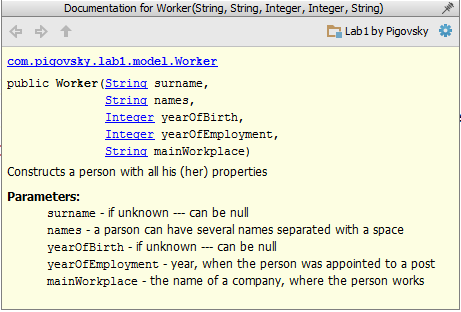
\includegraphics{JavadocExample}
\end{figure}

\item Потрібно створити JUnit тест-кейс, що перевіряє вірність роботи WorkerBuilder, тобто чи він дає вірні значення за замовчуванням для незаданих полів.
\end{enumerate}

JUnit тест можна створити натиснувши комбінацію клавіш <Ctrl>+<Shift>+<T>, перебуваючи у файлі з класом, до якого плануєте написати тест. Після цього, у контекстному меню, що появилося, слід натиснути ``Create new test''. 

У вікні створення теста оберіть JUnit4 навпроти Testing library. Ім'я класу залиште WorkerBuilderTest, назвою цільового пакету вкажіть com.<Ваше прізвище>.myapp.test. Поставте галочки навпроти setUp/@Before та у списку ``Generate test methods for:'' відзначте build(): Worker, як показано на рисунку
\begin{figure}[H]
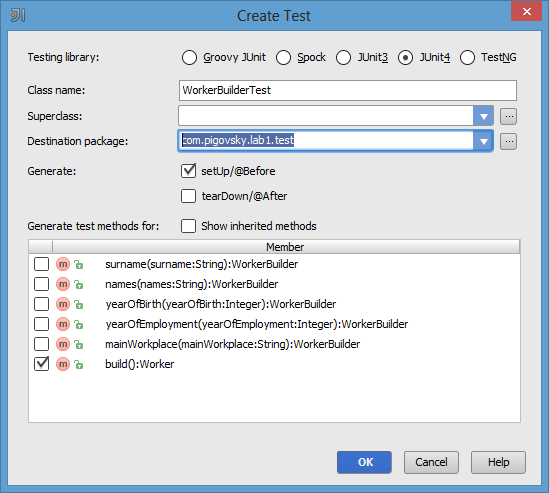
\includegraphics{createTest}
\end{figure}
Появиться вікно з текстом тесткейсового класу. Перш за все, після оголошення пакету, добавте оператор статичного імпортування функцій перевірки:
\begin{lstlisting}
import static org.junit.Assert.*;
\end{lstlisting}
Це дозволить звертатися до функцій на зразок Assert.assertEquals(...) за коротшим іменем assertEquals(...).

Метод setUp() буде викликатися перед запуском кожного тестового методу. Запишіть у ньому створення екземпляру об'єкта WorkerBuilder.

У методі testBuild задайте об'єкту-білдеру лише прізвище працівника (без року народження чи року прийняття на роботу) і побудуйте об'єкт працівника. Перевірте методом assertNull чи роки народження і прийняття на роботу мають очікуване неозначене null.
В результаті цих дій у Вас має утворитися щось на зразок нижчеподаного лістингу

\begin{lstlisting}
package com.pigovsky.lab1.test;

import com.pigovsky.lab1.model.Worker;
import com.pigovsky.lab1.model.WorkerBuilder;
import org.junit.Before;
import org.junit.Test;

import static org.junit.Assert.*;

/**
 * Tests if builder provides expected defaults
 */
public class WorkerBuilderTest {
    private WorkerBuilder builder;

    @Before
    public void setUp() throws Exception {
        builder = new WorkerBuilder();
    }

    @Test
    public void testBuild() throws Exception {
        Worker worker = builder.surname("Pigovsky").
                build();
        assertNull("Year of birth is not null, but " +
                "it should be null by default!",
                worker.getYearOfBirth());
        assertNull("Year of appointment is " +
                "not null, but it should be " +
                "null by default!",
                worker.getYearOfEmployment());
    }
}
\end{lstlisting}

Спробуйте запустити тест. Для цього Вам доведеться створити нову конфігурацію запуску і задати Test kind в положення ``All in package'', як показано на рисунку
\begin{figure}[H]
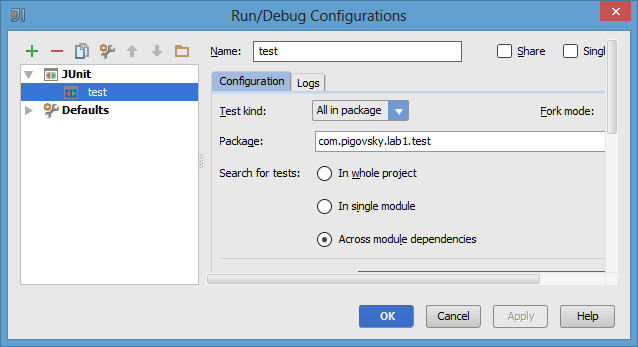
\includegraphics{testRunConfiguration}
\end{figure}

Тестування повинно пройти успішно, про що свідчитиме зелений progress bar. Після цього замініть значення років по-замовчуванню в класі WorkerBuilder на будь-що відмінне від неозначеного null, наприклад, на 0 (число нуль).
При повторному тестуванні, Ви мали би отримати повідомлення, схоже на ``java.lang.AssertionError: Year of appointment is not null, but it should be null by default!''.


В класі Worker cтворіть метод getAge(), який рахує вік працівника за роком народження. При цьому, треба бути завбачливим і врахувати, що Вашою програмою можуть користуватися більше як один рік. Тому для отримання поточного року використайте виклик на зразок
\begin{lstlisting}
int currentYear = Calendar.getInstance().get(Calendar.YEAR);
\end{lstlisting}

Для тестування методу getAge, створіть ще один тест-кейс, як Ви це вже робили для методу build. Приклад тест-кейсу наведено у лістингу:
\begin{lstlisting}
package com.pigovsky.lab1.test;

import com.pigovsky.lab1.model.WorkerBuilder;
import org.junit.Test;

import static org.junit.Assert.assertEquals;

/**
 * Tests if age is computed correctly
 */
public class WorkerTest {
    @Test
    public void testGetAge() throws Exception {
        assertEquals(32, new WorkerBuilder().
                yearOfBirth(1983).
                    build().
                        getAge());
    }
}
\end{lstlisting}

\subsection{Зміст звіту}

Звітом з виконання лабораторної роботи є файли проекту в оприлюдниному репозиторії (див. розділ {\bf Загальні принципи звітування і оцінювання лабораторних робіт з ``Технології Java''}.
 
